\documentclass[15pt]{extarticle}
\usepackage[a4paper, 
            hmargin=20mm, vmargin={20mm, 30mm}
            ]{geometry}
\usepackage{graphicx}
\usepackage[utf8]{inputenc}
\usepackage[T1]{fontenc}
\usepackage{lmodern}
\usepackage{titlesec}

\usepackage{natbib}
\bibliographystyle{copernicus}

\usepackage{tabularray}
\UseTblrLibrary{siunitx}

\usepackage{gensymb}

\usepackage{mathtools} % for \DeclarePairedDelimiter macro
\DeclarePairedDelimiter{\abs}{\lvert}{\rvert}


\titlespacing*{\section}
{0pt}{10.0ex plus 1ex minus .2ex}{2.0ex plus .1ex minus .1ex}
\titlespacing*{\subsection}
{0pt}{6.0ex plus 1ex minus .2ex}{1.0ex plus .1ex minus .1ex}

% For enumerations with section number.
%\usepackage{enumitem}
%\setenumerate[1]{label=\thesection.\arabic*.}
%\setenumerate[2]{label*=\arabic*.}


\renewcommand{\familydefault}{\sfdefault}


\usepackage[colorlinks = true,
            linkcolor = blue,
            urlcolor  = blue,
            citecolor = black,
            anchorcolor = blue]{hyperref}

\setlength{\parskip}{0.5em}
\renewcommand{\baselinestretch}{1.2}

\title{DMBSim v1.0: overview and model physics}
\author{Enrico Mattea}
\date{September 2021}


\begin{document}

%\maketitle

\begin{titlepage}
    
\includegraphics[width=5cm]{unifr_logo}
    \par
    \vspace{2.0cm}
	\centering
	{\huge\textbf{DMBSim v1.0\\}}
	\vspace{0.3 cm}
	{\large Model description and main equations\\}
	\vspace{1.6 cm}
	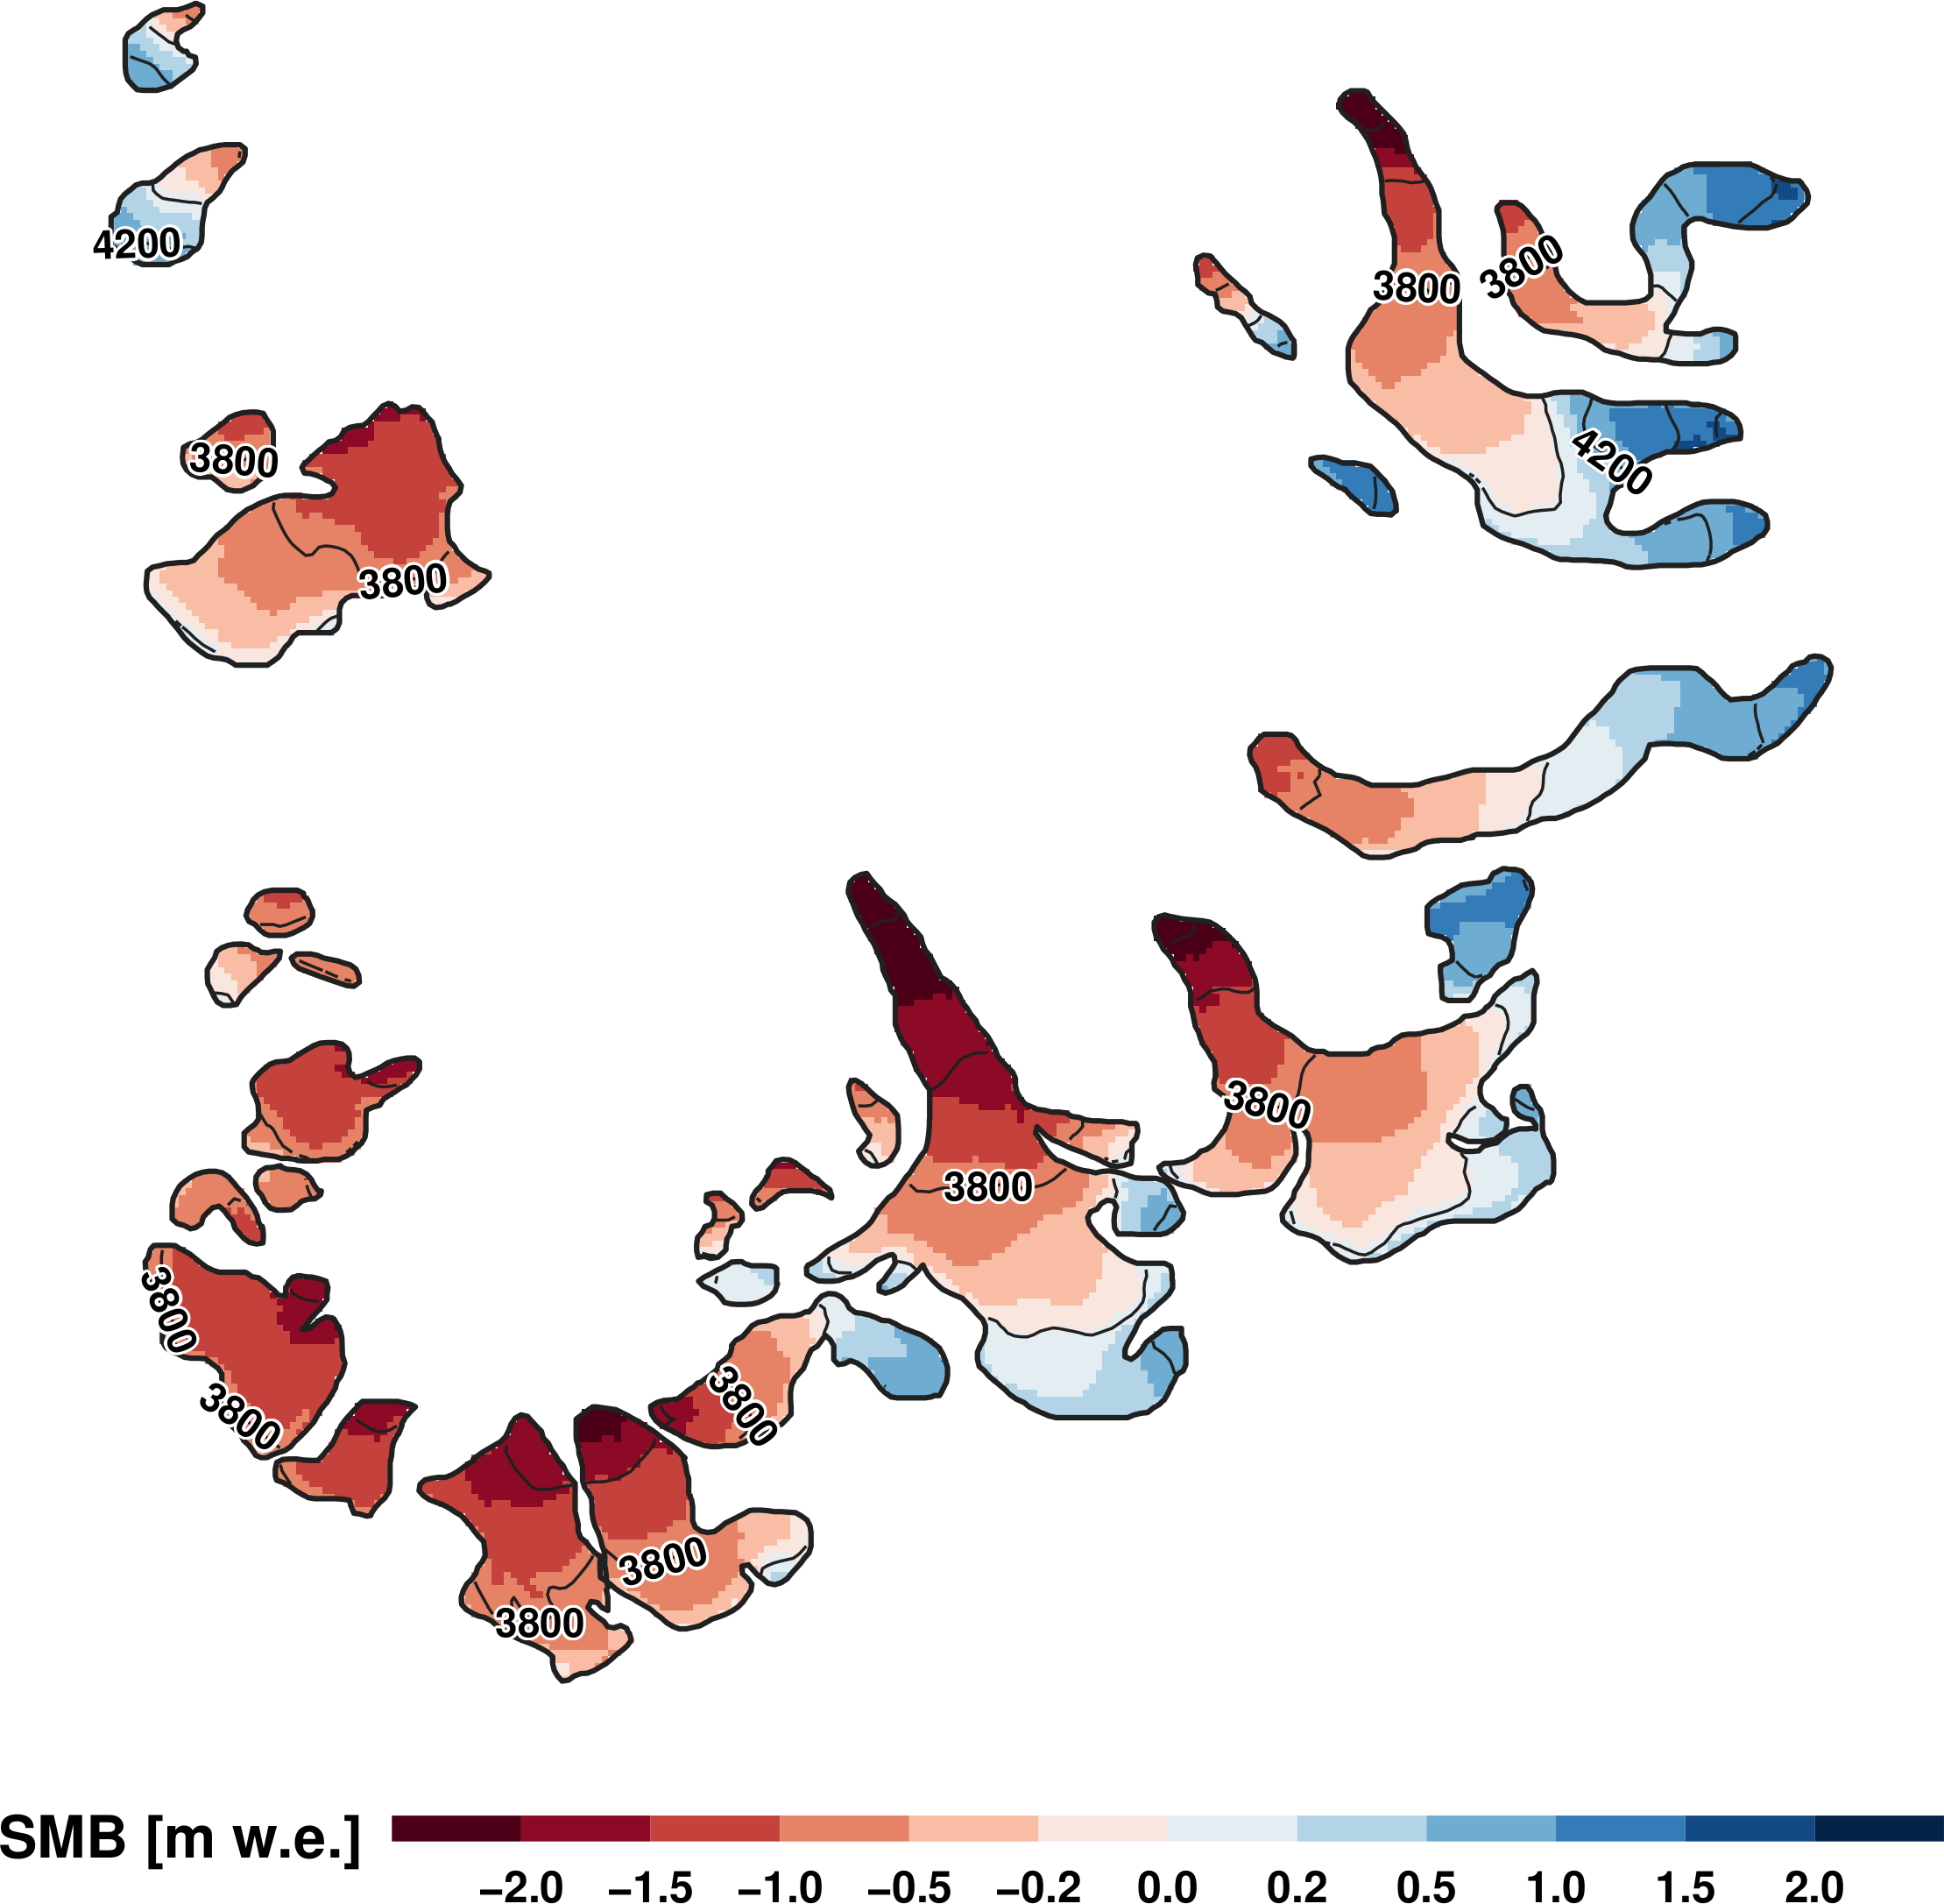
\includegraphics[width=12cm]{f0_cover_image}\par
	\vspace{1.45 cm}
	{\normalsize \textbf{Enrico Mattea}\\}
	{\normalsize \textit{enrico.mattea@unifr.ch\\}}
	\vspace{0.6 cm}
	{\normalsize October 2021}
	\vfill

\end{titlepage}


\section{Introduction}
\textbf{NOTE:} this document presents the model architecture and the main equations. If you want to start \textbf{using the model} right away, you may check out the \textbf{tutorials} instead.

\textbf{DMBSim} is a physical model of glacier \textbf{surface mass balance.} It simulates the mass balance of one or more glaciers based on \textbf{meteorological and topographic data.} Moreover, it can use \textbf{mass balance measurements} to calibrate automatically the parameters of the simulation. The \textbf{model output} consists of \textbf{maps and time series} of surface mass balance over different periods, such as the hydrological year and the winter season. The model is entirely written in the open-source \textbf{R} programming language and works on both Windows and Linux systems.

\section{Model description}
The simulation is performed \textbf{on a grid}, which is defined by a \textbf{digital elevation model} (DEM). Mass balance is driven by a \textbf{daily meteorological series} of mean daily \textbf{temperature} and total \textbf{precipitation}, and also a set of 365 grids of \textbf{potential incoming solar radiation.} The simulation can span \textbf{one or more years:} in the latter case, each year is modeled \textbf{individually} and can use different parameters from the others.

The model starts from an \textbf{initial condition} of snow-water equivalent (SWE). This can either be the result of the previous year of the simulation, or be computed automatically considering several factors: topography, snow line altitude, an elevation gradient, avalanches and optionally winter snow measurements. Then the model computes \textbf{daily accumulation and melt} for each grid cell, following the formulas in Table \ref{table:t1_massbal_model}: accumulation is gridded using an elevation gradient and topographic distribution grid, while melt is computed with an enhanced \textbf{temperature/radiation index} based on \citet{hock_distributed_1999}. The melt model can distinguish between snow, firn, bare ice and debris-covered ice (as provided in the input data), and also account for progressively darker ice towards the glacier terminus. Daily mass balance values are recorded over the course of the simulation period, to finally extract the \textbf{cumulative mass balance} at specific dates. Mass balance is also used to calculate derived values, such as the equilibrium line altitude (ELA), the accumulation-area ratio (AAR), and the daily discharge from the glacier. The model can simulate the occurrence of \textbf{avalanches}, which redistribute snow (also from/to non-glaciated terrain) with a process-based approach \citep{gruber_mass-conserving_2007}. The model automatically processes the DEM to ensure the correct hydrologic flow of avalanches.

If \textbf{mass balance measurements} are supplied (such as \textbf{stakes} or \textbf{snow pits}), the model \textbf{optimizes the parameters} over the corresponding observation periods, to find the best match with the measurements. Specifically, the melt factor and the radiation factors (see next section) are optimized \textbf{until the simulation is unbiased} (at the measured locations) compared to the measured values. If \textbf{winter snow measurements} are also supplied, the model will additionally optimize the precipitation correction factor (see next section). The \textbf{RMS error} is not considered in the optimizations, it can be reduced (if needed) by manually tuning the other model parameters (see \textbf{tutorials}). When measurements are supplied, the simulation of the corresponding year can last more than 365 days, to include both the hydrological year (1 October-30 September) and the measurement period. When the simulation is finished the model also computes a \textbf{"corrected" mass balance} distribution over each measurement period: the simulated mass balance is smoothly corrected within elevation bands, using the local bias with respect to the point measurements (similar to the \textbf{contour-line method:} \citeauthor{ostrem_glacier_1991}, \citeyear{ostrem_glacier_1991}).

The simulation of multiple years can use \textbf{different input DEMs and glacier outlines:} this is useful if the glacier shape or topography change during the modeled period (usually over 5 years or more). The model can also \textbf{interpolate} automatically between the elevation grids of different years.

\section{Model equations}
The mass balance model works with the following \textbf{main variables} to calculate the values of Table \ref{table:t1_massbal_model}:
\begin{itemize}
    \item $x$ and $y$ are the coordinates on the grid
    \item $z(x,y)$ is the altitude (in m above sea level) of the grid cell at coordinates $x$ and $y$
    \item $z_{AWS}$ is the altitude of the meteo station
    \item $T_{AWS}$ is the daily mean temperature (in \celsius) measured at the meteo station
    \item $P_{AWS}$ is the daily total precipitation (in mm w.e.) measured at the meteo station
    \item $Q(x,y)$ is the daily mean potential incoming solar radiation (in W m\textsuperscript{-2}) for the grid cell at coordinates $x$ and $y$
    \item $M_f$ is the melt factor (in mm w.e. \celsius\textsuperscript{-1} d\textsuperscript{-1}); it is constant over the glacier
    \item $r_i$, $r_f$ and $r_s$ are the radiation factors for ice, firn and snow (in 10\textsuperscript{-3} mm w.e. \celsius\textsuperscript{-1} h\textsuperscript{-1} (W m\textsuperscript{-2})\textsuperscript{-1}); they are constant over the areas covered by ice, firn and snow, and largest for ice, smallest for snow, intermediate for firn
    \item $a_i(x,y)$ is an ice albedo factor ($\geq$ 1, dependent on the altitude); it can be used to simulate the presence of darker ice (which melts faster) on the lower tongue of the glacier
    \item $f_{deb}$ is a reduction factor (between 0 and 1, constant over the entire glacier) for the melt of debris-covered ice, which melts more slowly
    \item $\frac{dT}{dz}$ is the temperature gradient (in \celsius / 100 m)
    \item $\frac{dP}{dz}$ is the precipitation gradient (in \% / 100 m)
    \item $c_p$ is the precipitation correction (in \%: 100 = no correction, 200 = 2x correction)
    \item $c_{ps}$ is a factor which can be used to reduce the precipitation correction in summer: it can be between 0 and 1 from May to September, it is always 1 in the other months
    \item $T_{r/s}$ is the temperature of transition between rainfall and snowfall (default 1.5 \celsius).
    \item $F_p(x,y)$ is a factor for the spatial distribution of snow, it is derived from the winter snow probes if available (else 1.0 everywhere).
    \item $F_t(x,y)$ is a factor for the spatial distribution of snow, it is derived from the DEM topography (less snow on the exposed ridges, more in the depressions).
    \item $z_{Pmax}$ is the altitude at which there is the maximum precipitation, then it does not increase further.
\end{itemize}



    \begin{table}[h!]
\caption{main quantities calculated by the model}
\label{table:t1_massbal_model}
\begin{tblr}{hline{1,2,Z},
             colspec = {Q[l,m,$] Q[c,m] X[1.3,l,m,$] X[0.7,j,m]},
             row{1} = {font=\bfseries,rowsep = 3pt},
             row{2-Z} = {rowsep = 5pt},
             column{2-Y} = {colsep = 9pt}
             }
\text{Symbol}
        & Unit  & \text{Equation}
                    & Explanation   \\
%
T(x,y)  & \celsius & T_{\mathit{AWS}} + \frac{dT}{dz} \cdot (z(x,y) - z_{\mathit{AWS}})
                       & \textbf{Air temperature} over each grid cell \\
%
P_{\mathit{AWS},\mathrm{corr}} & mm w.e. & P_{\mathit{AWS}} \cdot \frac{c_p}{100} \cdot c_{ps}
                       & \textbf{Corrected total precipitation} at the meteo station \\
%
P(x,y)  & mm w.e.       & F_p(x,y)F_t(x,y)P_{\mathit{AWS},\mathrm{corr}}\cdot \frac{dP}{dz}\cdot \newline
                  \cdot \bigl\{1 + [\min(z_{P_{\max}},z(x,y)) - z_{\mathit{AWS}}]\bigr\}/10000
                       & \textbf{Total precipitation} over each grid cell   \\
%
f_s(x,y)& --       &   \begin{cases}
                       1   & \text{if }T(x,y)\leq T_{r/s} - \qty{1}{\celsius} \\
                       \left[T_{r/s} + 1 - T(x,y)\right]/2
                       & \text{if }\abs{T(x,y) - T_{r/s}} < \qty{1}{\celsius} \\
                       0   & \text{if }T(x,y)\geq T_{r/s} + \qty{1}{\celsius}
                       \end{cases}
                       & Fraction of \textbf{solid precipitation} over each grid cell. It is linearly interpolated within \qty{\pm1}{\celsius} of $T_{r/s}$ \\
%
C(x,y) & mm w.e.        & P(x,y)\cdot f_s(x,y)
                       & \textbf{New snow accumulation} over each grid cell \\
%
m_i(x,y) & mm w.e.      & \left[M_f + \frac{24}{1000} \cdot r_i \cdot a_i(x,y) \cdot Q(x,y)\right] \cdot T(x,y)
                       & \textbf{Melt} amount for cells with an \textbf{ice} surface \\
%
m_f(x,y) & mm w.e.      & \left[M_f + \frac{24}{1000} \cdot r_f \cdot Q(x,y)\right] \cdot T(x,y)
                       & \textbf{Melt} amount for cells with a \textbf{firn} surface \\
%
m_f(x,y) & mm w.e.      & \left[M_f + \frac{24}{1000} \cdot r_s \cdot Q(x,y)\right] \cdot T(x,y)
                       & \textbf{Melt} amount for cells with a \textbf{snow} surface \\        
%
m_d(x,y) & mm w.e.      & f_{deb} \cdot \left[M_f + \frac{24}{1000} \cdot r_i \cdot Q(x,y)\right] \cdot T(x,y)
                       & \textbf{Melt} amount for cells with a \textbf{debris-covered} surface \\                          
\end{tblr}
    \end{table}
    

\vbox{
\section{Code architecture and folder structure}
The main model file is \textit{main.R}, it calls the functions located in folder \textit{functions\textbackslash}. These \textbf{function files} should not be modified when running the model; each file contains the definition of one function, with the same name as the file. Function files include many \textbf{comments} which explain in detail all the model calculations. The main \textbf{model parameters} (such as glacier name and modeled years) are set by editing file \textit{set\_params.R}; the procedure to set individual annual parameters is explained in \textbf{tutorial 2}. Some \textbf{advanced parameters} can be set in file \textit{functions\textbackslash func\_process\_run\_params.R}. \textbf{Note} that these advanced parameters can produce errors if set to a wrong value. Two \textbf{additional programs} are provided in folder \textit{utils\textbackslash}: file \textit{install\_packages.R} \textbf{to install the needed modules}, and file \textit{make\_input.R} \textbf{to prepare input data} in the correct format. Usage of these programs is explained in \textbf{tutorial 1}.
}
    
\bibliography{refs.bib}
\end{document} 
